% Paper draft. Build: latexmk -pdf main.tex (in paper/). Figures: python scripts/paper_figures.py.
% Numbers come from results/ (see the comment above each table); \todo marks what is still open.
\documentclass[11pt]{article}
\usepackage[margin=2.5cm]{geometry}
\usepackage[T1]{fontenc}
\usepackage[utf8]{inputenc}
\usepackage{lmodern}
\usepackage{amsmath}
\usepackage{booktabs}
\usepackage{graphicx}
\usepackage{siunitx}
\usepackage[authoryear,round]{natbib}
\usepackage[hidelinks]{hyperref}
\usepackage{xcolor}
\newcommand{\todo}[1]{\textcolor{red}{[TODO: #1]}}
\graphicspath{{figures/}}
\sisetup{detect-all}

\title{\todo{title}\\Untrained networks, wavelet scattering and pretrained models\\as frozen EEG feature extractors}
\author{Roy Seo$^{1}$, Yohan Chatelain$^{1,\dagger}$, Mina Alizadeh$^{2}$, Injy Fouda$^{3}$,
  Jishang Jiang$^{3}$, Tristan Glatard$^{1,5,6,\dagger}$\\[1ex]
  \small $^{1}$Krembil Centre for Neuroinformatics, Centre for Addiction and Mental Health, Toronto\\
  \small $^{2}$Department of Computer Science and Software Engineering,\\
  \small Gina Cody School of Engineering and Computer Science, Concordia University, Montreal\\
  \small $^{3}$Integrated Program in Neuroscience, Faculty of Medicine and Health Sciences,\\
  \small McGill University, Montreal, Canada\\
  \small $^{4}$Department of Neurology and Neurosurgery, McGill University, Montreal, Canada \todo{unused}\\
  \small $^{5}$Department of Psychiatry, University of Toronto, Toronto, Canada\\
  \small $^{6}$Department of Computer Science, University of Toronto, Toronto, Canada}
\date{}

\begin{document}
\maketitle

\begin{abstract}
\todo{draft, to rewrite once the discussion is settled}
Pretrained EEG models, including large foundation models, are usually compared with trained
baselines. We compare them with feature extractors that learn nothing: convolutional networks
with random weights and the wavelet scattering transform. All extractors are frozen and read
out by the same logistic-regression probe on ten classification tasks from six open datasets
(eyes closed vs open, depression, Alzheimer's disease, frontotemporal dementia, Parkinson's
disease, age, motor imagery and sleep staging). Pretrained EEGNet checkpoints gain at most
0.055 AUC over randomly initialized copies of the same network, less than the spread across
random seeds on all but one task. Single foundation models reach the highest AUC on most tasks,
but averaging the predictions of 30 untrained ShallowFBCSPNet instances closes most of the gap,
and no foundation model is significantly better than this ensemble; at these sample sizes the
two cannot be told apart, which does not make them equivalent. Single random initializations of the same network differ by up to 0.26 AUC on depression and
0.49 on Parkinson's disease, so untrained baselines should be reported over many seeds or as
ensembles.
\end{abstract}

\section{Introduction}
Pretrained EEG models now range from small supervised networks trained on one motor-imagery
dataset to self-supervised foundation models trained on thousands of hours of clinical
recordings \citep{kostas2021bendr, jiang2024labram, wang2024eegpt, wang2025cbramod}. These
models are evaluated by fine-tuning them or by fitting a probe on their frozen features, and they
are compared with supervised networks trained from scratch on the target task \citep{roy2019}.
That comparison measures the value of a pretrained model against task-specific training. It does
not measure what pretraining adds to the network itself: a frozen network with random weights also
produces features, shaped by its temporal convolutions, spatial mixing and pooling.

Random-weight networks are a strong baseline in other domains. In object recognition, random
convolutional filters followed by rectification and pooling reached accuracies close to those of
learned filters \citep{jarrett2009}, and the architecture alone accounted for much of the
performance of the learned network \citep{saxe2011}. Random features approximate kernel machines
\citep{rahimi2007}, and an untrained convolutional generator is a sufficient prior for image
restoration \citep{ulyanov2018}. \todo{cite untrained CNNs on 2D/3D neuroimaging (Chatelain et
al., 2026?).} The wavelet scattering transform gives a second reference that learns nothing and,
unlike a random network, has no seed: a cascade of fixed wavelet filters and modulus operators whose
averaged outputs are stable to small deformations \citep{mallat2012, anden2014}. We are not aware of
a comparison of pretrained EEG models with untrained networks and scattering under the same frozen
readout and across several tasks.

Such a comparison has to account for variability that a single trained baseline hides. The
features of an untrained network change with the random seed, so one seed can land well above or
below the typical result; seed variance is a known source of spurious differences between methods
\citep{bouthillier2021}. Clinical EEG datasets are small, and with tens of participants per group
the uncertainty of a cross-validated AUC is of the same order as the differences between methods
\citep{varoquaux2018}. A pretrained checkpoint or a foundation model is a single draw from its own
training process, whose variability is usually unknown.

We compare four kinds of frozen feature extractors: untrained convolutional networks (30 seeds
each), wavelet scattering, pretrained convolutional networks and seven foundation models (an eighth, BENDR, was left out: we could not reproduce its
pretraining input). Each is
read out by the same logistic-regression probe on ten classification tasks from six open datasets.
The design isolates the pretrained weights by pairing each pretrained network with untrained copies
of the same architecture fed the same input, measures the spread across seeds, checkpoints and
cross-validation splits, and compares single foundation models with ensembles of untrained instances.
Significance is tested with permutations that refit every instance's probe, so that the test of an
extractor uses all its instances rather than one chosen seed. Pretrained EEGNet weights improved the
AUC over their untrained twins by at most 0.055, and no foundation model was significantly better
than an ensemble of 30 untrained ShallowFBCSPNet instances.

\section{Methods}

\subsection{Datasets and tasks}
We evaluated all feature extractors on ten classification tasks drawn from six openly
available EEG datasets (Table~\ref{tab:tasks}). Each dataset is downloaded from its public
source. \todo{the ds002778 curators ask to be contacted before submission: confirm done.}

\begin{table}[t]
\centering\footnotesize\setlength{\tabcolsep}{4pt}
\caption{Tasks and datasets. Tasks 2 and 6 are each evaluated separately on eyes-closed and
eyes-open recordings, giving ten tasks.}
\label{tab:tasks}
\begin{tabular}{@{}rllllr@{}}
\toprule
\# & Task & Dataset & Sample & Classes & Size \\
\midrule
1 & Eyes closed vs open (positive control) & ds003478 & 1-min block & 2 & 113 participants \\
2 & High vs low BDI, eyes closed / open & ds003478 & participant & 2 & 74 low, 39 high \\
3 & Alzheimer's disease vs control & ds004504 & participant & 2 & 36 AD, 29 controls \\
4 & Frontotemporal dementia vs control & ds004504 & participant & 2 & 23 FTD, 29 controls \\
5 & Parkinson's disease (off med.) vs control & ds002778 & participant & 2 & 15 PD, 16 controls \\
6 & Young vs old, eyes closed / open & MPI-LEMON & participant & 2 & 137 young, 65 old \\
7 & Left vs right hand motor imagery & BNCI2014\_001 & trial & 2 & 9 subjects, 2,592 trials \\
8 & Sleep staging (W, N1, N2, N3, REM) & Sleep-EDF & 30-s epoch & 5 & 20 subjects, 5,767 epochs \\
\bottomrule
\end{tabular}
\end{table}

\paragraph{Depression (ds003478).} ``EEG: Depression rest'' \citep[OpenNeuro ds003478 v1.1.0,
CC0;][]{cavanagh_ds003478, cavanagh2019} contains 122 college-aged participants recruited
from undergraduate psychology courses at the University of Arizona from mass-screening Beck
Depression Inventory (BDI) scores, with the BDI re-administered at the laboratory session.
Following the original study, we excluded one participant (original ID 544) whose BDI was
unstable between screening and the laboratory session. Participants were labelled by laboratory
BDI with the original cut-offs (low: BDI~$\le 6$, $n = 74$; high: BDI~$\ge 17$, $n = 39$); the
eight participants with intermediate scores were excluded. The final sample has 113 participants
(age 18--24 years, $M = 18.93$, $SD = 1.21$, missing for one; 67 female, 46 male). Structured
clinical interviews were available only for 26 high-BDI participants (9 current major depressive
disorder, 8 past, 9 neither), so BDI was the only grouping variable. EEG was recorded with a
64-channel Neuroscan SynAmps2 system (500~Hz; ground AFz; online reference between Cz and CPz).
Each participant completed two resting recordings of about 6~min made of 1-min eyes-open and
eyes-closed blocks in counterbalanced order. We analysed run~1 only: it is available for all
participants, precedes the experimental task and is not affected by fatigue.

\paragraph{Other datasets.} ds004504 \citep{miltiadous2023} provides resting eyes-closed EEG
(19 channels, 500~Hz) of patients with Alzheimer's disease, frontotemporal dementia and healthy
controls; each task compares one patient group with the controls. ds002778
\citep{rockhill_ds002778, jackson2019, swann2015, george2013} provides resting EEG (32 scalp
channels, 512~Hz) of patients with Parkinson's disease, recorded off medication, and matched
controls; the task was kept despite its small size. For MPI-LEMON \citep{babayan2019} we used
the authors' preprocessed eyes-closed and eyes-open recordings (250~Hz; two participants at
100~Hz) of the 137 participants aged 20--35 and the 65 aged 55--80. BNCI2014\_001
\citep[BCI Competition IV 2a;][]{tangermann2012, jayaram2018} has 22 EEG channels at 250~Hz;
we used the left- and right-hand imagery trials of both sessions, pooled in each subject's
cross-validation. The competition's protocol trains on the first session and tests on the second,
so our AUCs are not comparable with published BCI~IV~2a results. Sleep-EDF
\citep[sleep cassette;][]{kemp2000, goldberger2000} was restricted to the first 20 subjects
(39 nights) and the Fpz--Cz and Pz--Oz derivations at 100~Hz; stages 3 and 4 were merged into N3,
and at most 30 epochs per stage and night were drawn with a fixed seed.

\subsection{Preprocessing}
Preprocessing used MNE-Python \citep{gramfort2013}. Unless stated otherwise, each recording was
restricted to its scalp channels (60 for ds003478, 19 for ds004504, 32 for ds002778, 22 for
BNCI2014\_001), re-referenced to the common average, band-pass filtered at 1--40~Hz, resampled to
128~Hz and cut into non-overlapping 2-s windows. For ds003478 the six 1-min blocks of run~1 were
located from the event triggers (30 windows each). The continuous recordings of ds004504,
ds002778 and LEMON were cut into 60-s segments of 30 windows. In LEMON, channels removed by the
authors (56--61 remain per file) were rebuilt by spherical-spline interpolation, giving 61
channels for everyone. For BNCI2014\_001 the imagery period (2--6~s after trial onset) gives two
windows per trial. Sleep-EDF kept its bipolar derivations, was band-pass filtered at 0.5--40~Hz
to keep slow waves, stayed at 100~Hz and used one 30-s window per scored epoch.

Each pretrained model received the input it was trained on (channels, sampling rate, filtering,
scaling; Section~\ref{sec:extractors}), and each pretrained CNN was paired with an untrained twin
of the same architecture receiving the identical input.

\subsection{Feature extractors}\label{sec:extractors}
All extractors were frozen: no weights were trained or fine-tuned in this study. They fall into
four groups.

\paragraph{Untrained CNNs.} We treat randomly initialized CNNs as fixed, random, nonlinear
measurement operators whose features reflect only the architecture's inductive biases (temporal
locality, weight sharing, spatial mixing, pooling) \citep{saxe2011}. We used (i) a small 1D CNN:
a temporal convolution over all channels (32 filters, kernel 25), ELU, average pooling by 4, a
second convolution (64 filters, kernel 11), ELU and a global average over time, giving 64
features; (ii) ShallowFBCSPNet \citep{schirrmeister2017} and (iii) EEGNet \citep{lawhern2018}
on all channels, without their classification layer. Both are plain PyTorch copies of the
braindecode~1.8.1 implementations, tested to give bit-identical outputs. To provide matched
baselines for the pretrained CNNs, we also used (iv) EEGNet restricted to C3, Cz and C4 and
(v) ShallowFBCSPNet with the BCI~IV~2a input of its pretrained checkpoints (22 channels, 4--38~Hz,
250~Hz, exponential moving standardization). Weights were drawn as in braindecode (Xavier-uniform
for the convolutions of ShallowFBCSPNet and EEGNet, PyTorch's default Kaiming-uniform for the
1D CNN) for 30 seeds (0--29). Models ran in evaluation mode (dropout off, batch normalization with
its initial running statistics).

\paragraph{Pretrained CNNs.} We used published braindecode checkpoints as released. Ten
EEGNetv4 checkpoints, each trained on one MOABB motor-imagery dataset, take C3, Cz and C4 at
128~Hz; two further checkpoints trained on another input scale (Cho2017, Ofner2017) were
excluded, and on motor imagery the checkpoint trained on BNCI2014\_001 was left out, leaving
nine. Their training band-pass is not published; they received our 1--40~Hz data. The checkpoints
differ in their pretraining data, not only in their random seed. Two
ShallowFBCSPNet checkpoints (braindecode tutorial models, both trained on subject 3 of
BNCI2014\_001) take the 22-channel BCI~IV~2a input; they were run on ds003478 only (not on BNCI2014\_001, their training data). The two differ in
their training recipe (trial-wise or cropped decoding).

\paragraph{Wavelet scattering.} As a fixed reference that is neither learned nor random, we
computed the 1D wavelet scattering transform \citep{mallat2012, anden2014} of each channel with
Kymatio \citep{andreux2020}: Morlet wavelets, orders 0--2, $Q = (8, 1)$, $\log(1 + x)$ applied to
orders 1 and 2, then averaged over time. Its only free parameter, the largest scale $J$
(averaging window about $2^J$ samples, 62~ms to 2~s at 128~Hz), took six values, $J = 3, \dots, 8$,
giving six instances.

\paragraph{Foundation models.} We evaluated the scalp-EEG foundation models whose weights are
open and load in braindecode~1.8.1: EEGPT \citep{wang2024eegpt}, LaBraM \citep{jiang2024labram},
BENDR \citep{kostas2021bendr}, CBraMod \citep{wang2025cbramod}, CodeBrain \citep{ma2026codebrain},
EEG-DINO small and medium \citep{wang2025eegdino} and Signal-JEPA \citep{guetschel2024sjepa}.
Models needing braindecode's development version (MIRepNet, BrainOmni) and models whose
pretraining corpus we could not check were not used; REVE was excluded because its weights
require registration (its corpus also includes ds002778). No model was evaluated on a dataset in
its pretraining data. Each model received its pretraining sampling rate, channel set and window
(30-s windows for CodeBrain; 256~Hz for EEGPT, as in the authors' code, where braindecode's model
card gives 250~Hz); CodeBrain and EEG-DINO need the 19 channels of the 10--20 system and
were not run on BNCI2014\_001, and no foundation model was run on Sleep-EDF's two bipolar
derivations. Features were averaged over time patches, keeping channels. EEGPT received millivolts,
as in the authors' pretraining script; BENDR's input scaling is not documented and was assumed
(per-channel min--max). Each foundation model is a single instance. We could not reproduce BENDR's
pretraining input: with ours its features were nearly constant across inputs (median SD across
blocks 0.0004, against 0.2--0.9 for EEGPT and LaBraM), which more likely reflects our input
scaling or the braindecode port than the model itself. It was left out of the ensemble pools and
of every test, a decision based on the features and not on the results; its AUCs are in
Table~\ref{tab:bendr}.

\paragraph{Feature counts.} The extractors give very different numbers of features: 64 for the
small 1D CNN, 128 for EEGNet, 440 for ShallowFBCSPNet (1,080 with the BCI~IV~2a input), 1,216 to
3,200 for Signal-JEPA, 2,048 for EEGPT, 3,800 to 12,200 for the other foundation models and 456
to 14,274 for scattering, depending on the scale and the number of channels.

\paragraph{Feature aggregation.} Window features were averaged within each 1-min block or 60-s
segment. For participant-level tasks they were then averaged over the participant's segments
(of one condition for the eyes-closed and eyes-open tasks), giving one feature vector per sample.
For motor imagery the two windows of a trial were averaged.

\subsection{Probe}
Every extractor was read out by the same probe: standardization (fitted within training folds)
and L2-regularized logistic regression ($C = 1$, L-BFGS, at most 5000 iterations;
scikit-learn, \citealp{pedregosa2011}), under stratified 5-fold cross-validation with one fixed
fold assignment shared by all extractors and instances. Folds kept all blocks of a participant
together for eyes closed vs open, and all epochs of a subject together for sleep staging
(stratified group $k$-fold). For motor imagery each subject had its own 5-fold cross-validation,
and the AUC was computed over all subjects' trials. We report the ROC AUC of the out-of-fold
predictions (macro one-vs-rest AUC for sleep staging) and the balanced accuracy.

With the same $C$ for 64 to 14,274 features and 31 to 202 participants, the effective
regularization differs between extractors. We therefore repeated phase~1 with two other probes,
both fitted within training folds with the same outer folds: $C$ chosen by an inner
cross-validation of the same kind ($C = 10^{-4}, \dots, 10^{2}$), and standardized features reduced
to 32 whitened principal components for every extractor (fewer when a training fold is smaller)
before the probe with $C = 1$.

\subsection{Sources of variability}
For each extractor we measured (i) instance variability, the SD of AUC across instances, and
(ii) split variability, the SD of AUC of one instance over 30 cross-validation fold assignments
(10 for sleep staging). An instance is not the same object for every kind of extractor, so
instance variability measures different sources: initialization alone for untrained networks
(30 seeds); pretraining dataset and training run for the EEGNetv4 checkpoints (10); training
recipe for the ShallowFBCSPNet checkpoints (2); and the choice of a hyperparameter for scattering
(6 scales $J$). It is not measured for foundation models, which have one public checkpoint each;
their variability across pretraining runs is unknown, not zero. Instance spreads are therefore
compared across kinds only with this difference in mind (Section~\ref{sec:matched}).

\subsection{Pretrained vs matched untrained networks}\label{sec:matched}
Each pretrained CNN was compared with its untrained twin (same architecture, channels and
preprocessing; only the weights differ). We report the gap (mean pretrained AUC minus mean
untrained AUC) and the share of untrained seeds that a checkpoint beats, averaged over
checkpoints (the normalized Mann--Whitney $U$; 50\,\% means no better than a random
initialization). The checkpoints' spread includes differences in pretraining data, so it is
expected to exceed what repeated pretraining on one dataset would give; the comparison asks whether
a checkpoint can be told apart from a random initialization, not whether the two spreads are
equal.

\subsection{Ensembles of instances}
For each pool of instances and ensemble size $K$ we drew up to 50 random subsets of $K$ instances
(20 for averaged features) and combined them by (i) averaging the out-of-fold predicted
probabilities, (ii) majority vote, with ties (even $K$) broken by the mean probability, or
(iii) averaging the features before fitting one probe per draw. Averaged features need instances
of one extractor with the same feature size, so they were computed on single-extractor pools
only (not on scattering, nor on Sleep-EDF where a probe per draw is too slow). Besides one pool per
extractor, we formed mixed pools: the three all-channel untrained architectures (1D CNN,
ShallowFBCSPNet, EEGNet), the pretrained CNNs, the foundation models, and all pretrained models.
We report the mean and SD of AUC across draws. Draws from a finite pool overlap more as $K$ grows
(a single subset exists at $K$ equal to the pool size), so the SD at large $K$ is a lower bound on
the variability of independent ensembles.

\subsection{Statistical tests}\label{sec:tests}
\paragraph{Primary test.} Does a typical instance of an extractor beat chance? For each
extractor and task, the probe of every instance was refit on the same shuffled labels, with the
same folds, and the median AUC over instances was compared with its null distribution
\citep{ojala2010}. Labels were shuffled within participant where a participant contributes several
samples (eyes closed vs open), within subject for motor imagery, and freely otherwise. Every
extractor of a task saw the same 10,000 shuffled labelings. The $p$-values were corrected for the
extractors of each task by the Westfall--Young step-down min-$P$ procedure \citep{westfall1993},
which uses these joint permutation nulls and therefore the correlation between extractors; it
controls the familywise error rate like Holm's procedure, with more power when the tests are
correlated. We report the corrected value as $p_\text{maxT}$. The family is one task's extractors: each task
asks its own question, and the familywise error rate is controlled within a task, not over the
whole study. This test was not run on Sleep-EDF,
where five-class probes are slow and every extractor is far above chance.

\paragraph{Secondary tests.} Each corrected per task: (1) the same refit permutation for the
ensemble of all instances (averaged predictions) and for the best instance (maximum over
instances, compared with the null maximum, so the choice of the best is accounted for);
(2) the refit permutation of each extractor's first instance alone (1,000 permutations, 200 for
sleep staging); (3) pretrained checkpoints vs the untrained seeds of the same architecture and
input (two-sided Mann--Whitney $U$); (4) each foundation model vs the averaged predictions of all
untrained ShallowFBCSPNet instances and of all scattering scales on the same samples (paired
permutation, 10,000 permutations shared by all pairs of a task, two-sided; the two models' scores
are swapped per sample, or per participant, all its samples together, where a participant
contributes several: eyes closed vs open and motor imagery). These two references were not fixed
before the study (there was no preregistration); Table~\ref{tab:fmpools} gives each foundation model
against the ensemble of every untrained network. Tests (1), (2) and (4) are corrected by max-$T$ as
above. Test (3) has no joint permutation null and is Holm-corrected \citep{holm1979}; it has one
comparison per task except on ds003478 (two). Scattering is not tested against the other
extractors: its scales $J = 3, \dots, 8$ are a design choice, not a random sample of instances, so
it is compared descriptively. Instance AUCs share the same samples, so tests (3) and (4) ask whether
the weights change the result beyond the weight-to-weight spread; they do not generalize to new
participants. Per-model tests decide whether each extractor beats chance; extractors are compared
with one another only through paired tests (3) and (4), never through their $p$-values.

\section{Results}

\subsection{Sample}
In ds003478 the low-BDI group had a mean BDI of 1.66 ($SD = 1.55$) and the high-BDI group 23.56
($SD = 4.00$). The groups did not differ in age ($t(110) = 0.69$, $p = .49$), but the high-BDI
group included more women (72\,\% vs 53\,\%; $\chi^2(1) = 3.86$, $p = .050$) and had much higher
trait anxiety (STAI 56.46 vs 30.88; Welch's $t = 20.64$, $p < .001$). Sample sizes of the other
datasets are in Table~\ref{tab:tasks}.

\subsection{The pipeline recovers a known effect}
On the positive control (eyes closed vs open) all groups of extractors performed well: wavelet
scattering reached a mean AUC of 0.973 over its six scales, untrained ShallowFBCSPNet 0.947 over
30 seeds, the pretrained ShallowFBCSPNet checkpoints 0.893 and the best foundation model
(CodeBrain) 0.984 (Table~\ref{tab:best}; Fig.~\ref{fig:phase1}). The median instance of every
extractor was above chance. The pipeline thus detects the well-known alpha increase
with eye closure, and near-chance results elsewhere are not due to a pipeline failure.

\begin{figure}[t]
\centering
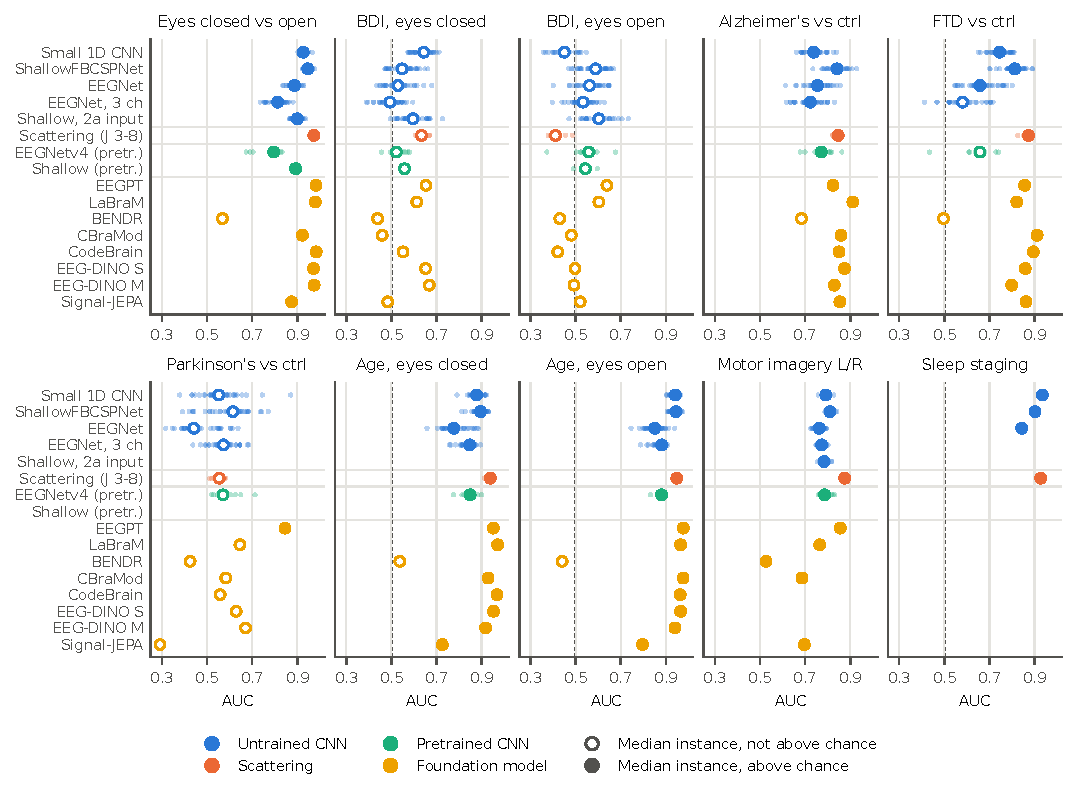
\includegraphics[width=\textwidth]{fig1_phase1}
\caption{AUC of every instance of every extractor on the ten tasks. Small dots: random seeds
(untrained CNNs), published checkpoints (pretrained CNNs) or scales $J$ (scattering); foundation
models have one checkpoint each. Large marker: median instance, filled when it beats chance (median
instance refit permutation, max-$T$ corrected per task; on sleep staging, where it was not run,
the first instance). Dashed line: chance. Empty rows: extractor not run on that dataset. BENDR,
left out of the analyses, is not shown.}
\label{fig:phase1}
\end{figure}

\subsection{Best extractor of each kind}
Table~\ref{tab:best} lists, for each task, the best extractor of each group (mean AUC over
instances; foundation models are single instances). The best single foundation model scored
highest on 8 of the 9 tasks where foundation models could be run; on motor imagery, scattering
(0.875) exceeded the best foundation model (EEGPT, 0.858). Scattering exceeded the best untrained
CNN on 7 of 10 tasks. The foundation-model column reports the maximum over seven models, whereas
the other columns report means over instances, which favours the foundation-model column.

% results/phase1/<dataset>/metrics.csv, cv_seed 0: mean AUC over instances, best per group.
\begin{table}[t]
\centering\footnotesize\setlength{\tabcolsep}{4pt}
\caption{Best extractor of each group per task (mean AUC over instances).}
\label{tab:best}
\begin{tabular}{@{}llllll@{}}
\toprule
Dataset & Task & Untrained CNN & Scattering & Pretrained CNN & Foundation \\
\midrule
ds003478 & Eyes closed vs open & ShallowFBCSPNet 0.947 & 0.973 & Shallow 0.893 & CodeBrain 0.984 \\
ds003478 & BDI, eyes closed & Small 1D CNN 0.636 & 0.638 & Shallow 0.558 & EEGPT 0.690 \\
ds003478 & BDI, eyes open & Shallow 2a 0.601 & 0.422 & EEGNetv4 0.547 & EEGPT 0.656 \\
ds004504 & AD vs control & ShallowFBCSPNet 0.839 & 0.844 & EEGNetv4 0.773 & LaBraM 0.912 \\
ds004504 & FTD vs control & ShallowFBCSPNet 0.808 & 0.864 & EEGNetv4 0.642 & CBraMod 0.912 \\
ds002778 & PD vs control & ShallowFBCSPNet 0.591 & 0.551 & EEGNetv4 0.589 & EEGPT 0.863 \\
LEMON & Young vs old, EC & ShallowFBCSPNet 0.891 & 0.936 & EEGNetv4 0.846 & LaBraM 0.971 \\
LEMON & Young vs old, EO & ShallowFBCSPNet 0.940 & 0.946 & EEGNetv4 0.877 & EEGPT 0.977 \\
BNCI2014\_001 & Left vs right MI & ShallowFBCSPNet 0.810 & 0.875 & EEGNetv4 0.793 & EEGPT 0.858 \\
Sleep-EDF & 5-stage (macro) & Small 1D CNN 0.935 & 0.929 & -- & -- \\
\bottomrule
\end{tabular}
\end{table}

The depression and Parkinson's tasks were near chance for most extractors. With the primary test,
79 of the 121 extractor $\times$ task tests were significant: all 11 on motor imagery, all 26 on
age, 25 of 26 on dementia, 16 of 45 on ds003478 and 1 of 13 on Parkinson's. On ds003478, 15 of
the 16 are on eyes closed vs open. We report depression as a null result: the sixteenth is the
only significant test of 30 on depression, and it is borderline: the small 1D CNN on BDI with eyes closed (median instance AUC 0.644, $p = 0.0036$,
$p_\text{maxT} = 0.042$). For the same extractor and task, the ensemble ($p_\text{maxT} = 0.093$)
and best-instance (0.24) statistics were not significant, nor was EEGPT, the best single model on
this task (AUC 0.690, $p_\text{maxT} = 0.067$). Nothing was significant on BDI with eyes open. The
ensemble and best-instance statistics otherwise agreed with the median, except EEGNet and the
EEGNetv4 checkpoints on FTD (significant for the ensemble and the median, not for the best
instance). On Parkinson's only EEGPT was significant (AUC 0.863, $p_\text{maxT} = 0.024$), while
Signal-JEPA scored well below chance (0.292); with $n = 31$ these results should be read with care.
Signal-JEPA's inversion is stable across 30 cross-validation splits (mean 0.26) and under both
alternative probes (0.28 and 0.34), so it is not an effect of weak regularization.

\subsection{Pretraining adds little over a matched random initialization}
Against untrained twins with identical architecture and input, the EEGNetv4 checkpoints improved
mean AUC on 8 of 9 tasks, by at most 0.055 (FTD; gaps $-0.039$ to $+0.055$; Table~\ref{tab:matched}).
The gap was smaller than the untrained seed SD on every task but motor imagery ($+0.021$ vs SD
0.015), and a checkpoint beat on average 30--75\,\% of the untrained seeds. The difference was
significant for Alzheimer's disease ($p_\text{Holm} = 0.021$) and motor imagery (0.029), borderline
for FTD (0.051) and not significant elsewhere ($p_\text{Holm} \ge 0.13$). The two ShallowFBCSPNet
checkpoints underperformed their twins on all three ds003478 tasks (gaps $-0.006$, $-0.037$,
$-0.057$; 25--45\,\% of seeds beaten; $p_\text{Holm} \ge 0.44$), although these single-subject tutorial
models are weakly pretrained.

% results/dashboard/p1_matched.csv and the vs_matched rows of results/stats/stats.csv.
\begin{table}[t]
\centering\footnotesize\setlength{\tabcolsep}{4pt}
\caption{Pretrained checkpoints vs their matched untrained baseline: mean AUCs, gap, SD of the
baseline over 30 seeds, share of seeds a checkpoint beats, and Mann--Whitney $p$, Holm-corrected
per task.}
\label{tab:matched}
\begin{tabular}{@{}lllrrrrrr@{}}
\toprule
Dataset & Pretrained & Task & Pretr. & Baseline & Gap & Seed SD & Beaten & $p_\text{Holm}$ \\
\midrule
ds003478 & EEGNetv4 & Eyes closed vs open & 0.771 & 0.810 & $-0.039$ & 0.037 & 30\,\% & 0.14 \\
ds003478 & EEGNetv4 & BDI, eyes closed & 0.528 & 0.494 & $+0.033$ & 0.052 & 70\,\% & 0.14 \\
ds003478 & EEGNetv4 & BDI, eyes open & 0.547 & 0.529 & $+0.018$ & 0.053 & 63\,\% & 0.46 \\
ds003478 & ShallowFBCSPNet & Eyes closed vs open & 0.893 & 0.899 & $-0.006$ & 0.019 & 45\,\% & 0.85 \\
ds003478 & ShallowFBCSPNet & BDI, eyes closed & 0.558 & 0.596 & $-0.037$ & 0.058 & 32\,\% & 0.44 \\
ds003478 & ShallowFBCSPNet & BDI, eyes open & 0.543 & 0.601 & $-0.057$ & 0.060 & 25\,\% & 0.46 \\
ds004504 & EEGNetv4 & AD vs control & 0.773 & 0.721 & $+0.052$ & 0.057 & 75\,\% & 0.021 \\
ds004504 & EEGNetv4 & FTD vs control & 0.642 & 0.587 & $+0.055$ & 0.079 & 71\,\% & 0.051 \\
ds002778 & EEGNetv4 & PD vs control & 0.589 & 0.574 & $+0.015$ & 0.062 & 54\,\% & 0.65 \\
LEMON & EEGNetv4 & Young vs old, EC & 0.846 & 0.838 & $+0.007$ & 0.033 & 56\,\% & 0.61 \\
LEMON & EEGNetv4 & Young vs old, EO & 0.877 & 0.873 & $+0.004$ & 0.028 & 51\,\% & 0.94 \\
BNCI2014\_001 & EEGNetv4 & Left vs right MI & 0.793 & 0.773 & $+0.021$ & 0.015 & 74\,\% & 0.029 \\
\bottomrule
\end{tabular}
\end{table}

\subsection{Probe regularization}
With $C$ chosen by inner cross-validation, the foundation models and scattering chose $C \approx
0.01$ (0.001 for EEGPT), a hundred times stronger regularization than the main probe, the small 1D CNN $C = 1$ and
EEGNet and ShallowFBCSPNet $C = 0.1$. The comparisons above held under both alternative probes. The
largest matched gap was 0.055 with $C = 1$, 0.042 with PCA and 0.028 with nested $C$. The best
foundation model's AUC minus that of the 30-seed ShallowFBCSPNet ensemble stayed between $-0.065$
and $+0.099$ on every task except Parkinson's, under all three probes. On Parkinson's EEGPT reached
0.863 with $C = 1$ and 0.879 with PCA but 0.650 with nested $C$, whose inner folds hold about five
participants: this result depends on the probe (Table~\ref{tab:probes}).

\subsection{Single-instance results are unstable}
Variability across random initializations was as large as or larger than the effects of interest.
For BDI with eyes closed, the untrained CNNs on all channels had seed SDs of 0.040--0.060 and
split SDs of 0.030--0.033; single seeds of EEGNet ranged from 0.435 to 0.680 AUC. Scattering was
the most stable extractor (SD 0.028 over its six scales). Foundation models, with one instance
each, still varied across cross-validation splits (SD 0.027--0.048), and their variability across
pretraining runs is unknown.

\subsection{Small ensembles of untrained networks approach foundation models}
Averaging the predictions of a few random instances raised the mean AUC and reduced its spread,
with most of the gain reached by $K \approx 5$--10 (Fig.~\ref{fig:ensembles}). On FTD vs control,
averaging the 30 untrained ShallowFBCSPNet seeds raised the AUC from 0.808 (mean single seed) to
0.861 at $K = 5$, 0.875 at $K = 10$ and 0.880 at $K = 30$, against 0.912 for the best foundation
model (CBraMod). On the nine tasks with foundation models, no foundation model was significantly
better than the 30-seed ShallowFBCSPNet ensemble ($p_\text{maxT}$ from 0.075 to 1 where the
foundation model scored higher, the lowest for EEGPT on Parkinson's); the 7 significant
differences all favoured the ensemble (EEGPT on motor imagery, 0.858 vs 0.902, was not significant
once the swaps kept each subject's trials together: $p_\text{maxT} = 0.24$). Against the scattering ensemble, four foundation-model
results were significantly better: EEGPT on Parkinson's ($p_\text{maxT} = 0.012$), EEGPT and
LaBraM on BDI with eyes open, where scattering is below chance (AUC 0.427; $p_\text{maxT} = 0.004$
and 0.008), and CodeBrain on age with eyes closed (0.969 vs 0.944, $p_\text{maxT} = 0.032$). With 52--65 participants on the dementia tasks, this means that the
foundation models and the untrained ensemble cannot be told apart at these sample sizes, not that
they are equivalent.

\begin{figure}[t]
\centering
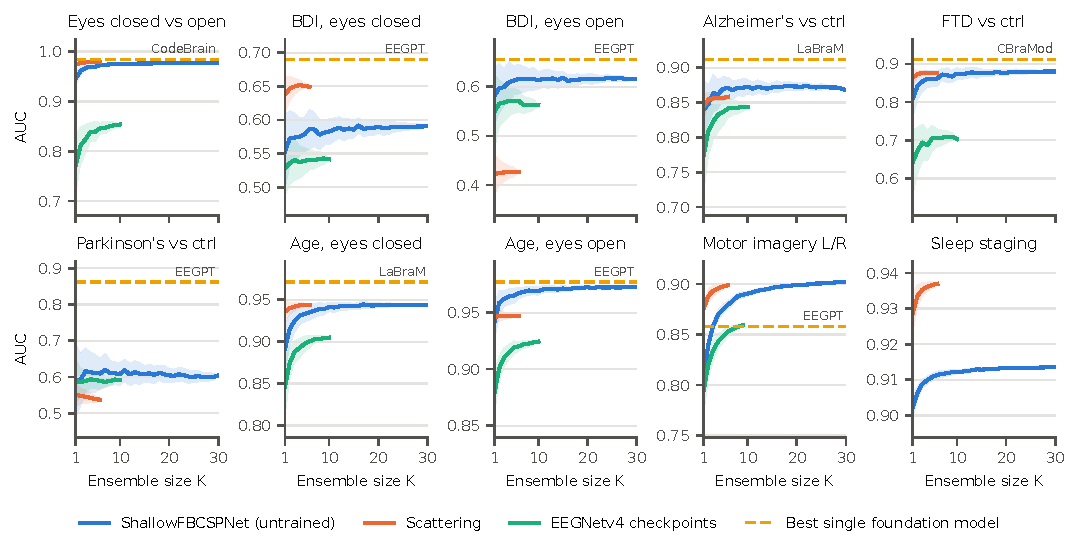
\includegraphics[width=\textwidth]{fig2_ensembles}
\caption{Mean AUC of ensembles of $K$ instances (averaged predictions) against $K$; band: SD over
draws (up to 50 per $K$), which shrinks at large $K$ partly because draws from a finite pool
overlap. Dashed line: best single foundation model, named in each panel.}
\label{fig:ensembles}
\end{figure}

% \subsection{Participant-level stability}  optional: per-sample score SD and disagreement across
% draws are in results/phase2/<dataset>/summary.csv (median_score_sd, disagreement).

\section{Discussion}

\paragraph{Pretrained weights add little to these architectures.} With architecture and input held
fixed, the EEGNetv4 checkpoints changed the AUC by $-0.039$ to $+0.055$ relative to random
initializations, within one seed SD on eight of nine tasks, and the difference was significant only
for Alzheimer's disease and motor imagery (Table~\ref{tab:matched}). Motor imagery is the task
closest to the checkpoints' training data, so the one gap larger than the seed SD is where transfer
is expected. The ShallowFBCSPNet checkpoints scored below their untrained twins on all three
ds003478 tasks. These results are consistent with the probe drawing most of its information from
what the architecture computes regardless of its weights: band-limited temporal filters, spatial
combinations of channels and pooled power. They bound the value of small supervised pretraining (one
motor-imagery dataset per EEGNetv4 checkpoint, one subject for ShallowFBCSPNet) and say nothing
about networks of the same size pretrained on large corpora, which we did not test.

\paragraph{Foundation models lead on single instances, not against ensembles.} The best single
foundation model had the highest AUC on 8 of the 9 tasks where foundation models ran
(Table~\ref{tab:best}), yet none was significantly better than the averaged predictions of 30
untrained ShallowFBCSPNet instances, and the 7 significant differences all favoured the ensemble.
Averaging the predictions of instances with different random weights reduces the variance that each
random feature map adds to the probe's output; most of the gain arrived by $K = 5$--10
(Fig.~\ref{fig:ensembles}). Scattering, a single deterministic transform, exceeded the best untrained
network on 7 of 10 tasks and every foundation model on motor imagery. Its largest margins over the
best untrained network were on motor imagery ($+0.065$), FTD ($+0.056$), age with eyes closed
($+0.045$) and eyes closed vs open ($+0.027$). Three of these four tasks have established spectral
markers (sensorimotor rhythms, age-related slowing, alpha power), which time-averaged scattering
coefficients summarize directly; this explanation is consistent with the data but was not tested
here.
Three features of our protocol may understate the foundation models. They were used frozen with
mean-pooled features, whereas most were designed to be fine-tuned; we could not reproduce
BENDR's pretraining input, so it could not be evaluated; and each model
received its pretraining sampling rate and channel set
through resampling and channel selection that may differ from its pretraining pipeline. Our results
therefore compare frozen representations under one linear readout. The comparison is also
asymmetric in the other direction: the foundation-model column of Table~\ref{tab:best} takes the
maximum over seven models chosen after the fact, while the other columns average over instances.

\paragraph{One seed is not a baseline.} On BDI with eyes closed, the AUC of single EEGNet seeds
ranged from 0.435 to 0.680, and on Parkinson's single 1D CNN seeds ranged from 0.379 to 0.871. A
study that reports one random initialization can therefore obtain almost any result in that range,
and a pretrained model compared with it can appear better or worse by chance. The choice of test
mattered as well. For the 30-seed 1D CNN ensemble on BDI with eyes closed, a label permutation that
did not refit the probe gave $p_\text{maxT} = 0.013$, while the refit permutation of the same
ensemble, which accounts for the probes having been fitted on the true labels \citep{ojala2010},
gave 0.093. The refit test of its median instance was borderline (0.042) and that of its best
instance was not significant (0.24). We suggest reporting untrained baselines as a distribution over seeds or as an ensemble, and
testing them with a refit permutation over all instances. The same reasoning applies to pretrained
models, whose variability we could measure only partly. The EEGNetv4 checkpoints vary in their
pretraining data as well as their seed, so their spread mixes two sources; each foundation model is
one draw from a pretraining run, and its variability across pretraining seeds is unknown. A single
foundation-model AUC is therefore subject to the same caution as a single-seed baseline, without a
way to quantify it from public checkpoints.

\paragraph{Clinical tasks near chance.} Depression is a null result: one test of 30 was
significant, and only just (the median instance of the small 1D CNN on BDI with eyes closed, $p_\text{maxT} = 0.042$); on
Parkinson's only EEGPT exceeded chance under the primary test, and its AUC depended on the probe
(0.650 with nested $C$). These are the smallest samples in the study. For
an AUC of 0.64 with 39 and 74 participants per group, the normal approximation of
\citet{hanley1982} gives a 95\,\% interval of about 0.53--0.75; for an AUC of 0.85 with 15 and 16
participants, about 0.71--0.99. Differences between extractors on these tasks are smaller than these
intervals, and Signal-JEPA's AUC of 0.292 on Parkinson's shows that a single model can also land far
below chance on 31 participants. The ds002778 curators advise against patient-vs-control claims from
that dataset alone; we report the Parkinson's results as a comparison between extractors on the same
samples, not as a biomarker.
On ds004504 the features carry the diagnosis, not the severity: regressing the MMSE score
succeeded across all participants, where the diagnosis alone explains 74\,\% of its variance, but
failed within patients for every extractor, including the Alzheimer's patients alone
(Supplement, Table~\ref{tab:mmse}).

\paragraph{Scope.} The conclusions hold for frozen features read out by a linear probe, with one
preprocessing pipeline per model and one fixed cross-validation split for the main results (the
split SD, 0.027--0.048 on BDI with eyes closed, is reported separately). The tests other than the
primary one condition on the observed samples: they ask whether the weights change the result beyond
the spread across instances, not whether the result would generalize to new participants. Leakage
was checked against the pretraining corpora that the model authors published; models whose corpora we
could not verify were left out, which excludes several recent foundation models. Sleep-EDF was
evaluated with untrained networks and scattering only.

On these ten tasks, a frozen untrained network averaged over a few dozen random initializations
reached AUCs that no foundation model exceeded significantly, and a fixed wavelet transform was
significantly exceeded in 4 of 60 comparisons with foundation models. Pretrained
EEG models should therefore be compared with untrained instances of their own architecture and with
scattering, and every such comparison should report the variability across instances.

\section*{Data and code availability}
All datasets are openly available (Table~\ref{tab:tasks}). The code, configurations and the
scripts that produce every number and figure are at
\url{https://github.com/royjoysoy/untrained_eeg_fuzzy_pytorch} (MIT license).
\todo{tag a release and cite its DOI.}

\section*{Acknowledgements}
\todo{Brainhack Montreal 2026; computations on Rorqual (Calcul Qu\'ebec, Digital Research
Alliance of Canada).}

\bibliographystyle{plainnat}
\bibliography{references}

\clearpage
\appendix
\renewcommand{\thetable}{S\arabic{table}}
\setcounter{table}{0}
\section*{Supplementary material}

\paragraph{BENDR.} Table~\ref{tab:bendr} gives BENDR's AUCs. We could not reproduce its
pretraining input: with our input (per-channel min--max, an assumption) its features were nearly
constant across inputs (median SD across blocks 0.0004, against 0.2--0.9 for EEGPT and LaBraM), so it was
left out of the ensemble pools and of every test (Section~\ref{sec:extractors}).

% results/phase1/<dataset>/metrics.csv, extractor bendr: fixed split, and SD over 30 CV splits.
\begin{table}[h]
\centering\footnotesize\setlength{\tabcolsep}{4pt}
\caption{BENDR: AUC at the fixed split and SD over 30 cross-validation splits.}
\label{tab:bendr}
\begin{tabular}{@{}lrr@{}}
\toprule
Task & AUC & Split SD \\
\midrule
Eyes closed vs open & 0.568 & 0.007 \\
BDI, eyes closed & 0.439 & 0.052 \\
BDI, eyes open & 0.430 & 0.031 \\
AD vs control & 0.684 & 0.021 \\
FTD vs control & 0.496 & 0.064 \\
PD vs control & 0.425 & 0.073 \\
Young vs old, EC & 0.537 & 0.019 \\
Young vs old, EO & 0.440 & 0.040 \\
Left vs right MI & 0.527 & 0.006 \\
\bottomrule
\end{tabular}
\end{table}

\paragraph{Probe regularization.} Table~\ref{tab:probes} repeats the two comparisons of the main
text under the three probes. With nested cross-validation the median chosen $C$ over tasks was 1
for the small 1D CNN; 0.1 for EEGNet (all channels and three channels), ShallowFBCSPNet and the
EEGNetv4 checkpoints; 0.01 for scattering and the foundation models except EEGPT (0.001); and
0.001 to 0.006 for ShallowFBCSPNet with the BCI~IV~2a input and its pretrained checkpoints.

% results/phase1 (C = 1) and results/sensitivity/{pca,nested}/<dataset>/: median instance.
\begin{table}[h]
\centering\footnotesize\setlength{\tabcolsep}{4pt}
\caption{The main comparisons under three probes: $C = 1$, PCA to 32 whitened components, and
$C$ chosen by inner cross-validation. Left: EEGNetv4 checkpoints minus their untrained twins (mean
AUC). Right: best foundation model (median instance) minus the 30-seed ShallowFBCSPNet ensemble.}
\label{tab:probes}
\begin{tabular}{@{}lrrrrrr@{}}
\toprule
& \multicolumn{3}{c}{Matched gap} & \multicolumn{3}{c}{Best FM $-$ ensemble} \\
\cmidrule(lr){2-4}\cmidrule(l){5-7}
Task & $C = 1$ & PCA & nested & $C = 1$ & PCA & nested \\
\midrule
Eyes closed vs open & $-0.039$ & $-0.038$ & $-0.049$ & $+0.007$ & $+0.000$ & $+0.003$ \\
BDI, eyes closed & $+0.033$ & $+0.016$ & $+0.006$ & $+0.099$ & $+0.076$ & $+0.066$ \\
BDI, eyes open & $+0.018$ & $-0.012$ & $+0.003$ & $+0.041$ & $+0.028$ & $+0.008$ \\
AD vs control & $+0.052$ & $+0.032$ & $+0.003$ & $+0.044$ & $+0.022$ & $+0.002$ \\
FTD vs control & $+0.055$ & $+0.035$ & $+0.028$ & $+0.031$ & $+0.070$ & $+0.025$ \\
PD vs control & $+0.015$ & $+0.040$ & $-0.005$ & $+0.258$ & $+0.238$ & $+0.075$ \\
Young vs old, EC & $+0.007$ & $+0.012$ & $+0.004$ & $+0.027$ & $+0.022$ & $+0.015$ \\
Young vs old, EO & $+0.004$ & $-0.001$ & $+0.001$ & $+0.005$ & $+0.001$ & $-0.001$ \\
Left vs right MI & $+0.021$ & $+0.042$ & $+0.028$ & $-0.044$ & $-0.037$ & $-0.065$ \\
\bottomrule
\end{tabular}
\end{table}

\paragraph{Foundation models against single seeds.} The paired test compares one foundation
model with an ensemble of 30 instances, which favours the ensemble by construction.
Table~\ref{tab:fmseeds} compares each foundation model with the single untrained ShallowFBCSPNet
seeds instead.

% results/stats/fm_vs_seeds.csv (ref shallow): share of the 30 seeds whose AUC the FM exceeds.
\begin{table}[h]
\centering\footnotesize\setlength{\tabcolsep}{3.5pt}
\caption{Share (\%) of the 30 untrained ShallowFBCSPNet seeds whose AUC each foundation model
exceeds (ties count half). --: not run.}
\label{tab:fmseeds}
\begin{tabular}{@{}lrrrrrrrrr@{}}
\toprule
& EC/EO & BDI EC & BDI EO & AD & FTD & PD & Age EC & Age EO & MI \\
\midrule
EEGPT & 100 & 100 & 90 & 43 & 77 & 100 & 100 & 100 & 100 \\
LaBraM & 100 & 83 & 57 & 97 & 60 & 65 & 100 & 93 & 0 \\
CBraMod & 3 & 0 & 3 & 70 & 100 & 43 & 93 & 100 & 0 \\
CodeBrain & 100 & 50 & 0 & 60 & 100 & 37 & 100 & 88 & -- \\
EEG-DINO S & 97 & 97 & 10 & 77 & 90 & 55 & 100 & 93 & -- \\
EEG-DINO M & 97 & 100 & 10 & 43 & 40 & 77 & 80 & 43 & -- \\
Signal-JEPA & 0 & 13 & 20 & 62 & 90 & 0 & 0 & 0 & 0 \\
\bottomrule
\end{tabular}
\end{table}

\paragraph{Motor imagery per subject.} Each subject has its own probe, so the AUC over all
subjects' trials mixes the calibrations of nine probes. Table~\ref{tab:misubject} gives the
per-subject AUC; the order of the extractors is the same.

% results/phase1/bnci2014_001/metrics.csv: auc_subject_mean, auc_subject_sd (median instance).
\begin{table}[h]
\centering\footnotesize\setlength{\tabcolsep}{4pt}
\caption{Left vs right hand motor imagery: AUC per subject (mean and SD over the 9 subjects) and
AUC over all trials, median instance.}
\label{tab:misubject}
\begin{tabular}{@{}lrrr@{}}
\toprule
Extractor & Per subject & SD & All trials \\
\midrule
Scattering & 0.866 & 0.104 & 0.876 \\
EEGPT & 0.831 & 0.135 & 0.858 \\
ShallowFBCSPNet & 0.797 & 0.121 & 0.810 \\
Shallow, 2a input & 0.771 & 0.129 & 0.784 \\
Small 1D CNN & 0.771 & 0.120 & 0.792 \\
EEGNetv4 & 0.769 & 0.120 & 0.786 \\
EEGNet, 3 ch & 0.759 & 0.113 & 0.773 \\
LaBraM & 0.754 & 0.130 & 0.765 \\
EEGNet & 0.754 & 0.094 & 0.763 \\
Signal-JEPA & 0.692 & 0.093 & 0.697 \\
CBraMod & 0.684 & 0.080 & 0.686 \\
\bottomrule
\end{tabular}
\end{table}

\paragraph{Uncertainty of the ranking.} Table~\ref{tab:ranks} gives, for each task, the three
extractors with the highest mean AUC, with the share of 1,000 bootstrap resamples in which each
ranks first and its 95\,\% rank interval. A resample draws participants (subjects for motor
imagery) with replacement and, for extractors with several instances, instances with replacement.
The probe is not refit in each resample, so the intervals are somewhat too narrow; foundation
models, with one instance, get no instance resampling.

% results/stats/ranking_<dataset>.csv, statistic mean (scripts/ranking.py).
\begin{table}[h]
\centering\footnotesize\setlength{\tabcolsep}{3pt}
\caption{Top three extractors per task by mean AUC: share of resamples ranked first, 95\,\% rank
interval.}
\label{tab:ranks}
\begin{tabular}{@{}llll@{}}
\toprule
Task & First & Second & Third \\
\midrule
Eyes closed vs open & CodeBrain (59\,\%, 1--4) & EEGPT (25\,\%, 1--4) & LaBraM (11\,\%, 1--5) \\
BDI, eyes closed & EEGPT (53\,\%, 1--6) & EEG-DINO M (21\,\%, 1--7) & EEG-DINO S (11\,\%, 1--8) \\
BDI, eyes open & EEGPT (67\,\%, 1--5) & LaBraM (11\,\%, 1--9) & Shallow, 2a input (9\,\%, 1--8) \\
AD vs control & LaBraM (78\,\%, 1--3) & EEG-DINO S (9\,\%, 1--9) & CBraMod (1\,\%, 2--8) \\
FTD vs control & CBraMod (52\,\%, 1--6) & CodeBrain (26\,\%, 1--5) & Scattering (3\,\%, 1--8) \\
PD vs control & EEGPT (98\,\%, 1--1) & EEG-DINO M (2\,\%, 2--10) & LaBraM (0\,\%, 2--10) \\
Young vs old, EC & LaBraM (58\,\%, 1--4) & CodeBrain (35\,\%, 1--4) & EEGPT (3\,\%, 1--5) \\
Young vs old, EO & EEGPT (45\,\%, 1--4) & CBraMod (41\,\%, 1--4) & EEG-DINO S (10\,\%, 1--6) \\
Left vs right MI & Scattering (81\,\%, 1--2) & EEGPT (19\,\%, 1--3) & ShallowFBCSPNet (0\,\%, 3--5) \\
Sleep staging & Small 1D CNN (95\,\%, 1--2) & Scattering (5\,\%, 1--2) & ShallowFBCSPNet (0\,\%, 3--3) \\
\bottomrule
\end{tabular}
\end{table}

\paragraph{Choice of the reference ensembles.} The ShallowFBCSPNet and scattering ensembles were
not fixed before the study. Table~\ref{tab:fmpools} gives the ensemble of every untrained network
and the number of foundation models above it. The ShallowFBCSPNet ensemble had the highest AUC of
the four untrained networks on 7 of the 9 tasks (exceptions: the 1D CNN ensemble on BDI with eyes closed and, by 0.0002,
on age with eyes closed), so it is the hardest of them for the foundation
models; against the weaker ensembles more foundation models score higher (no test).

% results/stats/fm_vs_seeds.csv, ref_ensemble_auc and fm_auc (scripts/stats.py).
\begin{table}[h]
\centering\footnotesize\setlength{\tabcolsep}{3pt}
\caption{AUC of the ensemble of all instances (averaged predictions) of each untrained extractor,
with the number of the 7 foundation models whose AUC is higher, and the best foundation model.
$^a$Four foundation models were run on motor imagery.}
\label{tab:fmpools}
\begin{tabular}{@{}lllllll@{}}
\toprule
Task & 1D CNN & EEGNet & EEGNet, 3 ch. & Shallow & Scattering & Best FM \\
\midrule
Eyes closed vs open & 0.952 (5) & 0.934 (5) & 0.868 (7) & 0.977 (3) & 0.979 (3) & CodeBrain 0.984 \\
BDI, eyes closed & 0.674 (1) & 0.584 (4) & 0.518 (5) & 0.591 (4) & 0.649 (3) & EEGPT 0.690 \\
BDI, eyes open & 0.438 (6) & 0.595 (2) & 0.539 (2) & 0.615 (1) & 0.427 (6) & EEGPT 0.656 \\
AD vs control & 0.770 (7) & 0.841 (5) & 0.778 (7) & 0.868 (2) & 0.858 (3) & LaBraM 0.912 \\
FTD vs control & 0.783 (7) & 0.771 (7) & 0.642 (7) & 0.880 (2) & 0.877 (2) & CBraMod 0.912 \\
PD vs control & 0.562 (5) & 0.446 (6) & 0.579 (5) & 0.604 (4) & 0.537 (6) & EEGPT 0.863 \\
Young vs old, EC & 0.944 (4) & 0.902 (6) & 0.895 (6) & 0.944 (4) & 0.944 (4) & LaBraM 0.971 \\
Young vs old, EO & 0.965 (3) & 0.947 (5) & 0.920 (6) & 0.972 (2) & 0.947 (5) & EEGPT 0.977 \\
Left vs right MI$^a$ & 0.883 (0) & 0.864 (0) & 0.822 (1) & 0.902 (0) & 0.899 (0) & EEGPT 0.858 \\
\bottomrule
\end{tabular}
\end{table}

\paragraph{Dementia severity (MMSE).} On ds004504 we also regressed the Mini-Mental State
Examination score (0--30) on the same frozen features, one sample per participant: across all 88
participants, across the 59 patients (Alzheimer's disease and FTD), and across the 36 Alzheimer's
patients alone. Every control scores 30, so the first task largely repeats the diagnosis (the
group alone explains 74\,\% of the MMSE variance); AD and FTD also differ in MMSE (24\,\% of the
variance among patients), so the patient task partly repeats AD vs FTD, and the Alzheimer's task
removes both. The probe was standardization and ridge regression with 5-fold cross-validation on
the dataset's fixed split. Unlike the classifier's fixed $C = 1$, the ridge penalty was chosen in
each training fold (leave-one-out over $10^{-2}, \dots, 10^{6}$), because $R^2$ depends on the scale
of the predictions, which an unsuited penalty ruins. The primary test was the same as for
classification: the median $R^2$ over instances against 10,000 refits on shuffled scores, max-$T$
corrected over the extractors of each task. Under shuffled scores $R^2$ is well below 0, so a
small positive $R^2$ can be significant. MMSE was predicted across all participants by 10 of 13
extractors and by none within patients or within Alzheimer's patients, where every extractor's
$R^2$ was below 0 (Table~\ref{tab:mmse}).

% results/stats/regression_ds004504.csv, statistic median (scripts/regression.py).
\begin{table}[h]
\centering\footnotesize\setlength{\tabcolsep}{4pt}
\caption{MMSE regression on ds004504: median $R^2$ over instances and $p_\text{maxT}$ (10,000 refit
permutations, max-$T$ per task).}
\label{tab:mmse}
\begin{tabular}{@{}lrrrrrr@{}}
\toprule
& \multicolumn{2}{c}{All ($n = 88$)} & \multicolumn{2}{c}{Patients ($n = 59$)} & \multicolumn{2}{c}{AD only ($n = 36$)} \\
Extractor & $R^2$ & $p_\text{maxT}$ & $R^2$ & $p_\text{maxT}$ & $R^2$ & $p_\text{maxT}$ \\
\midrule
Small 1D CNN & $0.082$ & 0.003 & $-0.090$ & 0.981 & $-0.103$ & 0.846 \\
EEGNet & $-0.005$ & 0.076 & $-0.074$ & 0.953 & $-0.058$ & 0.604 \\
EEGNet (3 ch.) & $-0.025$ & 0.400 & $-0.083$ & 0.968 & $-0.145$ & 0.891 \\
ShallowFBCSPNet & $0.169$ & 0.001 & $-0.196$ & 0.998 & $-0.070$ & 0.669 \\
Scattering & $0.179$ & 0.002 & $-0.183$ & 0.998 & $-0.108$ & 0.826 \\
EEGNetv4 (pretrained) & $-0.105$ & 0.957 & $-0.131$ & 0.998 & $-0.082$ & 0.749 \\
EEGPT & $0.031$ & 0.043 & $-0.194$ & 0.998 & $-0.178$ & 0.891 \\
LaBraM & $0.205$ & 0.001 & $-0.189$ & 0.998 & $-0.081$ & 0.749 \\
CBraMod & $0.149$ & 0.003 & $-0.122$ & 0.991 & $-0.106$ & 0.846 \\
CodeBrain & $0.206$ & 0.002 & $-0.123$ & 0.991 & $-0.108$ & 0.846 \\
EEG-DINO S & $0.060$ & 0.024 & $-0.228$ & 0.998 & $-0.118$ & 0.846 \\
EEG-DINO M & $0.064$ & 0.023 & $-0.113$ & 0.984 & $-0.149$ & 0.891 \\
Signal-JEPA & $0.212$ & 0.001 & $-0.156$ & 0.997 & $-0.017$ & 0.336 \\
\bottomrule
\end{tabular}
\end{table}
\end{document}
